%****************************************************************
% Chapter X
%****************************************************************
\label{chapter-performance}
\chapter{Performance}

%****************************************************************
What is great about the Android runtime is that most of the stress of memory reclamation is done for developers. The system will track what developers are doing and when it sees that an object is not needed anymore, it will free it on their behalf. However, this does not exclude performance problems from happening here. When the amount of memory have allocated reaches an upper limit, a Garbage Collection (GC) event will be kicked off to free any resources that might not be needed any longer, freeing up space for future allocations. 

Anytime the frame drips about the $16$ milliseconds barrier, and the users are going to start to notice \ref{fig:16ms-per-frame}. So any code that forces allocated memory to spike above this threshold can cause problems. For instance, memory can become tighter, if the developer is allocating and freeing a large number of objects in a short period of time, the temporary objects again kicking off GC event. As result, increasing the risk of Memory leaks. They are objects which the application is no longer using, but the garbage collector fails to recognize them as unused.

\begin{figure}[H]
\caption{16ms Per Frame}
\label{fig:16ms-per-frame}
\centering
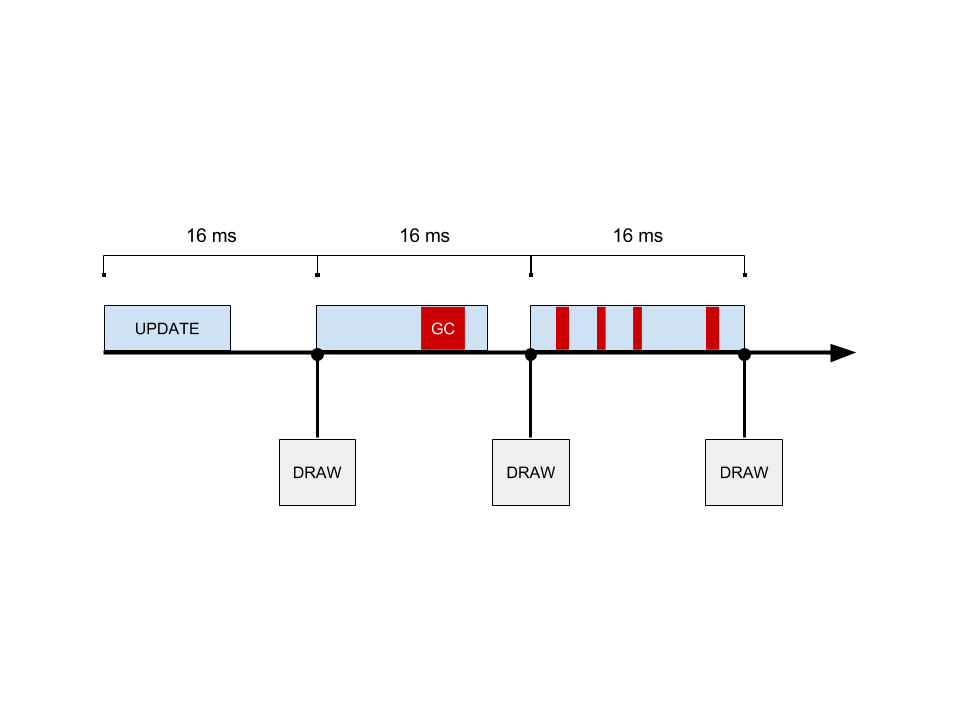
\includegraphics[width=\textwidth, keepaspectratio]{Figures/16ms-per-frame.png}
\decoRule
\end{figure}

Therefore, a performance testing is important for avoiding nasty GC events. Each GC event that developer can avoid, the application has more time per frame to do interesting things. In order to find out where in the code objects are being created but not released, created and not used, or created new when the developer could have been reusing them from existing objects. Android Studio provides a series of performance testing tools, such as Memory Monitor, Allocation Tracker, Heap Viewer, and the Systrace (it is an Android system trace tool helps developers analyze how the execution of the application fits into the many running systems on an Android device \cite{google.systrace.2016}).

%****************************************************************




%****************************************************************
The application has $55$ to $60$ FPS when the there is less than 250 \code{Placemark} exist in the scene. Although, the space partition that optimizes the intersection test has been significantly improved the performance. However, there is a performance limitation of current implementation due to the expensive render call in Android OpenGL ES API. It has a high priority and needs to be solved by calling the function once for all the same objects (\code{Placemark}).

%****************************************************************